%------------------------------------------------------------------------------
% Tema 6. Hemoglobina i ferro
%------------------------------------------------------------------------------
\section{Hemoglobina i ferro}

\subsection{La hemoglobina}
La hemoglobina és una proteïna globular que dona la coloració vermella
de la sang. Responsable del transport de \ch{O2}. Té un pes de  64,45
kDa.

Els nivells normals són de 16g/100 mL en homes i de 14g/100 mL en les dones.

Un home de 70 kg té 900 g d'hemoglobina. El bescanvi d'hemoglobina és
de 0,3 g/h (sintetitzats i destruïts).

Classificació de les malalties relacionades amb la hemoglobina:
\begin{itemize}
\item Reaccions de l'hemoglobina
  \begin{itemize}
  \item Metahemoglobinèmia hereditària
  \end{itemize}

\item Síntesi de la globina
  \begin{itemize}
  \item Hemoglobinopaties estructurals
    \begin{itemize}
    \item Anèmies drepanocítiques 
    \item Metahemoglobinèmia congènita
    \item Eritrocitosis (alterada afinitat per O2)
    \end{itemize}
  \item Talassèmies (hemoglobines alterades)
    \begin{itemize}
    \item  $\alpha$-talassèmies
    \item $\beta$-talassèmies
    \end{itemize}
  \end{itemize}

\item Síntesi i degradació del grup hemo
  \begin{itemize}
  \item Porfiries agudes
    \begin{itemize}
    \item Porfíria aguda intermitent 
    \item Coproporfíria hereditària
    \item Porfíria variegata
   \end{itemize}
  \item Porfíries no agudes
    \begin{itemize}
    \item Porfíria eritrohepàtica (eritropoiètica) 
    \item Porfíria eritropoiètica congènita
    \item Porfíria congènita (Intoxicació per plom)
    \end{itemize}
  \end{itemize}

\item Alteracions del metabolisme del ferro
  \begin{itemize}
  \item Anèmia ferropènica (manca de ferro)
    \begin{itemize}
    \item Pèrdua crònica de sang
    \item Ingesta inadequada de ferro
    \end{itemize}
  \item Anèmia sideroblàstica (mala utilització del ferro)
  \item Hemocromatosis (sobrecàrrega de ferro)
  \end{itemize}
\end{itemize}

\subsubsection{Estructura}
Hi ha 6 tipus de globines, que en la seva combinatòria generen els
diferents tipus d'hemoglobina que trobem en humans. Aquests tipus són:
$\alpha$, $\beta$, $\gamma$, $\delta$, $\epsilon$, $\zeta$.

La hemoglobina és un heterotetràmer $\alpha_2\beta_2$ en adults. Presenta
cooperativitat amb l'oxigen. També té al·losterisme amb el
2,3-difosfoglicerat, un intermediari de la glicòlisi que només es
troba en eritròcits. Això facilita l'alliberació d'oxigen als
teixits.

Es sintetitza als reticulòcits (eritròcits immadurs).

La hemoglobina presenta diferents subunitats segons l'estadi de
desenvolupament de l'individu:
\begin{itemize}
\item Adult:
  \begin{itemize}
  \item Hemoglobina A1 ($\alpha_2\beta_2$)
  \item Hemoglobina A2 ($\alpha_2\delta_2$)
  \end{itemize}

\item Fetal: Cadenes $\alpha_2\gamma_2$

\item Embrió:
  \begin{itemize}
  \item Grower I: $\zeta_2\epsilon_2$
  \item Grower II: $\alpha_2\epsilon_2$
  \item Portland: $\zeta_2\gamma_2$
  \end{itemize}
\end{itemize}

Hi ha 2 loci d' $\alpha$-globina al cromosoma 16 i un locus de $\beta$-globina
al cromosoma 11.

\subsection{Trastorns deguts a reaccions de l'hemoglobina}
La carboxihemoglobina presenta menys afinitat per l'hemoglobina.

\begin{figure}[H]
  \centering
  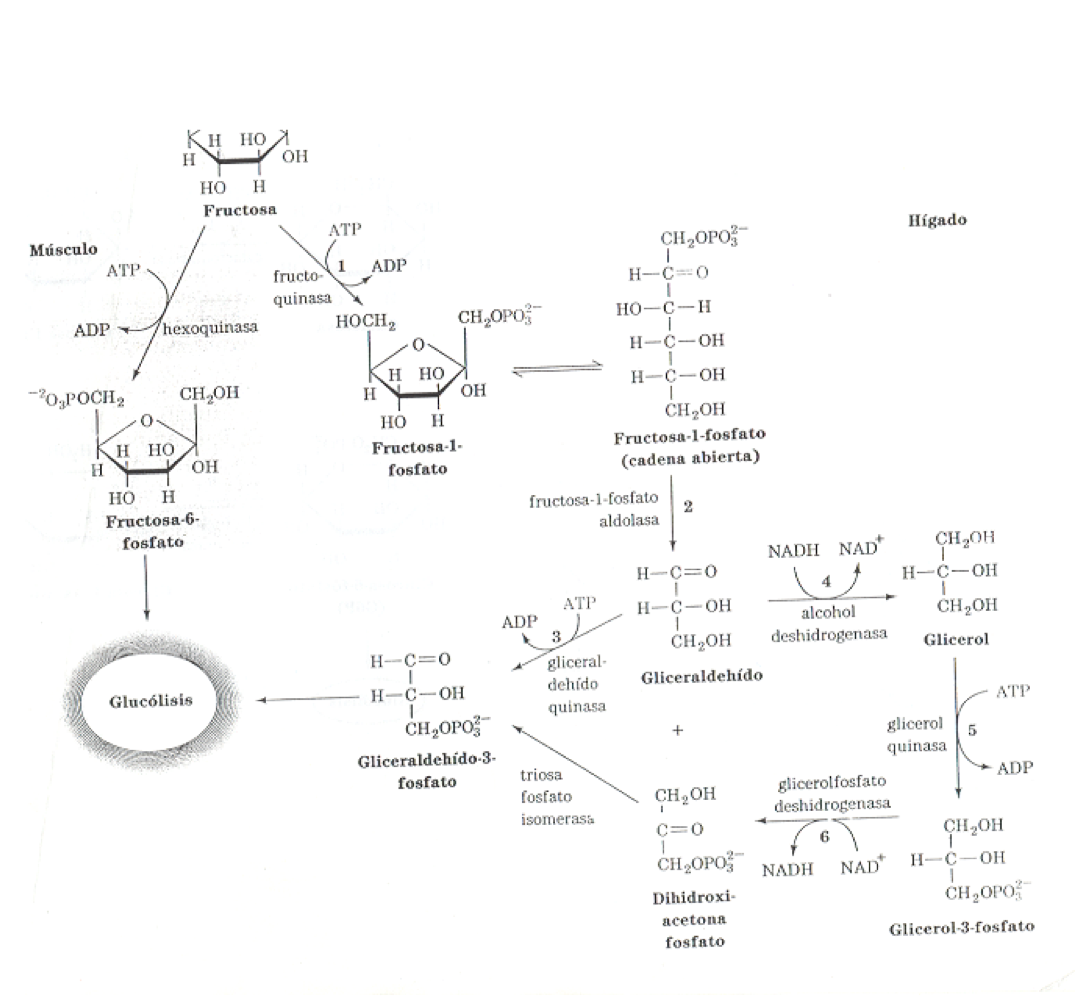
\includegraphics[width=0.5\textwidth]{fig5}
\end{figure}

Molt fàrmacs o agents oxidants poden provocar la formació de
metahemoglobina (amb \ch{Fe3+}), que mitjançant la NADH-metahemoglobina
reductasa la torna a reduir.

\begin{figure}[H]
  \centering
  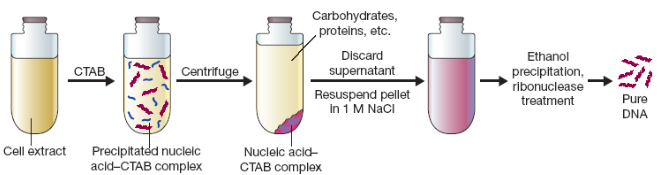
\includegraphics[width=0.5\textwidth]{fig6}
\end{figure}

La metahemoglobinèmia hereditària és una deficiència en NADH-metahemoglobina
reductasa. El Fe del hemo s'oxida en 25 \% a \ch{Fe3+} Es manifesta amb
cianosi (coloració fosca a la pell). Es tracta amb fàrmacs que
redueixin lametahemoglobina. És una malaltia
molt greu.

\subsection{Trastorns a la síntesi de la globina}
\subsubsection{Hemoglobinopaties estructurals}
Les mutacions perjudicials desapareixen, però les altres poden sobreviure
(els heterozigots resisteixen més que els homozigots). Algunes
mutacions són inòcues.

\paragraph{Hemoglobina S. Anèmia drepanocítica} \hfill \\
Es dóna un canvi d'aminoàcid Glu->Val a la cadena beta. És insoluble a baixes pressions
de \ch{O2}. Els glòbuls vermells presenten una morfologia
falciforme. Quan està desoxigenada, la hemoglobina es polimeritza i es
deformen els eritròcits. Els heterozigots  presenten poques vegades símptomes greus

Es va originar a Africa i confereix resistència a la malària. La
presenten un 40 \% de la població africana i un 10\% dels negres
americans.

La Hb pot polimeritzar formant fibres de 3000 \AA{}. Hi ha cicles
successius de forma de falç i normal. La forma de falç es trenca als
capil·lars per falta de flexibilitat. L'anèmia s'agreuja amb oxidants.

Altes concentracions d'HbS d'afinitat baixa per \ch{O2} no donen cap
problema fins l'administració d'un agent oxidant.

L'anèmia és menys severa si és dependent d'HbF. Els pacients tendeixen
a augmentar la proporció d'HbF en l'adult. Els homozigots d'Orient
Mitjà són asimptomàtics ja que tenen un 18\% d'HbF.

El diagnòstic es fa per electroforesi de la hemoglobina o per examen
microscòpic d'un frotis de sang.

Encara no hi ha tractament, encara que hi ha fàrmcs en estudi. La
profilaxi es basa en una bona nutrició i higiene, contra la
malària. En cas d'infecció, s'actua sobre l'agent infecciós. Si es fa
una transfusió quan es dona la primoquina ja que és oxidant i es pot
agreujar l'anèmia.

\paragraph{Hemoglobinopaties inestables} \hfill \\
S'han descrit més de 100 hemoglobinopaties. Es produeix la formació de
cossos d'inclusió intraeritrocítics (cossos de Heinz), que són
precipitacions d'hemoglobina. Consisteix en una sèrie de petites
granulacions que se situen a la perifèria dels hematies. Es produeix
en malalties congènites.

\begin{figure}[H]
  \centering
  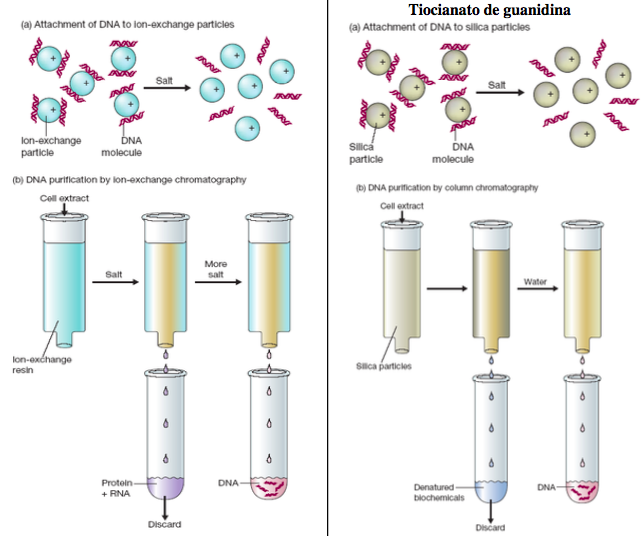
\includegraphics[width=0.8\textwidth]{fig7}
  \caption{Composició parcial en aminoàcids en la cadena $\beta$ humana
    normal i algunes hemoglobines amb cadenes $\beta$ anormals. Altres
    hemoglobines tenen cadenes $\alpha$ anormals.}
  \label{fig:fig7}
\end{figure}

\paragraph{Eritrocitosis} \hfill \\
Alteració en l'afinitat per \ch{O2}. En casos lleus no requereix
farmacologia. L'afinitat és més alta degut a canvis que eviten la unió
de 2,3-difosfoglicerat. Es produeix una hipòxia lleu (augment
d'eritròcits).

\paragraph{Metaglobinèmia} \hfill \\
Alteració en l'afinitat per \ch{O2}. Augmenta la metaglobulina (que és
hemoglobina amb \ch{Fe^3+}). Els eritròcits perden la capacitat de
transportar \ch{O2} i produeix cianosis.

Ens podem trobar:
\begin{itemize}
\item Metaglobinèmia adquirida: Produïda per fàrmacs, oxidants...

\item Metaglobinèmia congènita: Per deficiència de la
  citocrom-b5-reductasa o en presència d'hemoglobina M.
\end{itemize}

Hi ha Hb inestables, com la M que s'oxiden molt fàcilment a
\ch{Fe^3+}. Hi ha 5 tipus d'hemoglobina M, són mutacions al centre de
la unió de la globina al grup hemo. No hi ha afectació en
heterozigosi. L'homozigositat hauria de ser letal però no ho és.

Les manifestacions clíniques són:
\begin{itemize}
\item Cuanosi amb 1.5-2 g d'HbM (malaltia congènita del cor hi ha
  cianosi amb 5g d'Hb desoxigenada/100 mL)
\item Cianosi en el naixement en HbM de cadena alfa.
\item Cianosi als 6 mesos si el defecte està en beta.
\item És convenient fer el diagnòstic per descartar cianosi d'origen
  cardíac, que és molt greu.
\end{itemize}

\subsubsection{Talassèmies}
Són malalties en les que hi ha deficiència de globina, la poca que hi
ha és normal. Les causes són:
\begin{itemize}
\item Deleció gènica
\item Defectes en el processat de RNA
\item Mutacions sense sentit
\item Mutacions stop
\end{itemize}

Les beta talassèmies són més greus perquè només hi ha un locus de
cadena beta-globina.

\paragraph{beta-Talassèmies} \hfill \\
La síntesi de la cadena beta està disminuïda o és nul·la. No està
alterada la síntesi de la cadena alfa.

\begin{itemize}
\item $\beta^0$-talassèmia: No hi ha síntesi de cadena beta de la globina
  (augmenta la $HbA_2$). En homozigots, la HbF i HbA2 està augmentada;
  tenen anpemia microcítica hipocròmica i els eritròcits tenen mida i
  forma normals. Els heterozigots són asimptomàtics.

\item $\beta^+$-talassèmia: Síntesi de la cadena beta disminuïda
  (augmenta la HbA2). Els homozigots tenen els mateixos símptomes que
  l'anterior.

\item $\delta\beta$-talassèmia: Síntesi de la cadena beta i delta de
  globina disminuïdes. La gravetat depèn de si està compensada per una
  síntesi de cadena gamma.

\item $\gamma\delta\beta$-talassèmia: No hi ha síntesi de cadena gamma i
  delta i la cadena beta està disminuïda.
\end{itemize}

\paragraph{$\alpha$-Talassèmies} \hfill \\
Alterada la síntesi de la cadena $\alpha$. Es sinetteitzen en excés les
cadenes gamma (hemoglobina de Bart) i les cadenes beta (hemoglobina
H).

\begin{itemize}
\item alpha^0-Talassèmia: No hi ha síntesi de la cadena alfa de
  globina. La hemoglobina de Bart (tetràmer de delta) representa el 80
  90 \% de la hemoglobina total. És mortal ja que la HbBart no pot
    transportar O2.

  \item alpha^+-Talassèmia: 

  \item Hemoglobinopatia H: 
\end{itemize}

\paragraph*{Estudi bioquímic} \hfill \\
L'estudi de les hemoglobines s'efectua aprofitant la seva mobilitat
electroforètica:
\begin{itemize}
\item Fracció de metahemoglobina: En situacions normals, representa
  menys del 1,5 \% de la hemoglobina en sang. En el cas de la
  metahemoglobinèmia per deficiència de citocrom-b5-reductasa augmenta
  un 10-30 \%.

\item Fracció d'hemoglobina F: En situacions normals representa menys
  de l'1 \% de la hemoglobina en adult.


\end{itemize}


\subsection{Desordres de la síntesi del grup hemo}
La síntesi del grup hemo té lloc un 85\% en eritròcits i un 15\% en el
fetge.

La biosíntesis del grup hemo parteix de succinil-CoA i
glicina. Alteracions en la síntesi del grup hemo produeixen porfíries.

\subsubsection*{Síntesi del grup hemo}


\subsubsection*{Degradació del grup hemo}


\subsection{Alteracions del metabolisme del ferro}

\subsubsection{Anèmia ferropènica}


\subsubsection{Anèmia sideroblàstica}


\subsubsection{Hemocromatosis}